\documentclass[a4paper,10pt]{scrartcl}
\usepackage[utf8]{inputenc}
\usepackage[T1]{fontenc}
\usepackage[naustrian]{babel}
\usepackage{lmodern}
\usepackage{graphicx}
\usepackage{hyperref}
\usepackage{alltt}
\renewcommand{\ttdefault}{txtt}

%\usepackage{tabularx}
%\usepackage{amsmath}
%\usepackage{multirow}

%opening
\title{HCI Meilenstein 4}
\subtitle{Elektronisches Curriculum}
\author{Team 1 \\Pascal Attwenger, Philipp Hiermann, Sandra Markhart}

\begin{document}

\maketitle

\section{Einleitung}

Im Verlauf der letzten Wochen wurde in Gruppenarbeit ein neues Interface für die Prüfungsleistungen und das Mittelungsblatt (,,eCurriculum`) entwickelt.
Ziel dieser Studie ist es zu überprüfen, ob unser neues Interface wirklich besser zu bedienen ist als das alte Interface.

\section{Studienaufbau} 

Die Studie vergleicht unser neues Interface mit dem altem Interface (univis/Mitteilungsblatt). Die Aufgaben werden zuerst mit dem jeweils alten System durchgeführt und in Folge dessen in Hinblick auf die Bedienbarkeit mit dem neuen System verglichen.

Zusätzlich werden Fragebögen nach Vorbild von AttrackDiff verwendet, um die subjektive Zufriedenheit der Benutzer mit den Systemen festzuhalten.

\subsection{Hypothesen}


\begin{description}
 \item[Nullhypothese 1: ] User können mit unserem neu erstellten Interface Aufgaben schlechter oder gleich gut lösen als mit dem alten Interface. 
 \item[Alternativhypothese 1: ] User können mit unserem neu erstellten Interface Aufgaben besser lösen als mit dem alten Interface. 
\end{description}

\begin{description}
 \item[Nullhypothese 2: ] User sind mit unserem neu erstellten Interface weniger zufrieden oder gleich zufrieden als mit dem alten Interface. 
 \item[Alternativhypothese 2: ] User sind mit unserem neu erstellten Interface zufriedener als mit dem alten Interface. 
\end{description}


\subsection{Testbare Aufgaben}

\begin{description}
 \item[Aufgabe 1:] Welche Lehrveranstaltungen können im Modul ``Modul VMI Vertiefung Medieninformatik'' absolviert werden? (Mitteilungsblatt)
 \item[Aufgabe 2:] Wieviele ECTS bringt die UE Arbeitstechniken Multimediajournalismus? (Mitteilungsblatt)
 %\item Wieviele ECTS habe ich in meinem Studium bereits absolviert?
 %\item Wieviele Module habe ich bereits in meinem Studium abgeschlossen?
 \item[Aufgabe 3:] Welche Note habe ich in der Übung ``UE Technische Grundlagen und Systemsoftware''? (univis)
\end{description}

\subsection{Variablen}

\subsubsection{Performanzmetriken}

\begin{itemize}
 \item Zeit in Sekunden
 \item Anzahl der Klicks bei den univis-Aufgaben (deprecated)
\end{itemize}

\subsubsection{Subjektives Nutzerfeedback}

Ein AttrakDiff-Fragebogen, bei dem folgende Eigenschaften mit 7 verschiedenen Möglichkeiten zu bewerten sind:

\begin{itemize}
\item einfach - kompliziert 
\item menschlich - technisch
\item verständlich - unverständlich
\item übersichtlich - unübersichtlich 
\item innovativ - konservativ
\item kreativ - phantasielos
\item schön - hässlich
\item fröhlich - deprimierend 
\end{itemize}

\begin{description}
 \item[Datei auf cewebs:] Meilenstein 4 -- Team 1 -- Fragebogen
\end{description}

\subsection{Pre-Test}

In Folge des Pre-Tests mussten wir feststellen, dass die Variable ``Klicks'' nicht zielführend war,
da in den meisten Fällen nur ein Klick benötigt wurde, weshalb diese in der späteren tatsächlichen Studie weggelassen wurde.

Die restlichen Daten waren jedoch hinsichtlich ihrer Eignung für die Studie nicht beeinflusst und konnten daher weiterverwendet werden.

\subsection{Testpersonen}

\begin{description}
 \item[RL:] männlich, 21, studiert Rechtswissenschaften an der JKU Linz
 \item[JM:] männlich, 21, studiert Rechtswissenschaften an der JKU Linz
 \item[MS:] männlich, 21, studiert Informatik an der JKU Linz
 \item[JF:] weiblich, 14, Schülerin
 \item[NM:] weiblich, 47, noch nie mit dem Univis gearbeitet
 \item[DK:] männlich, 27, studiert Medieninformatik an der Uni Wien
 \item[JB:] weiblich, 30, studierte 4 Semester Psychologie an der Uni Wien
 \item[PH:] männlich, 27, studiert Medieninformatik an der Uni Wien
\end{description}

\subsection{Methodik}

Bei der Auswahl der Testpersonen wurde darauf geachtet, eine ausgewogene Mischung verschiedenster Studienhintergründe zu erreichen: Es wurden sowohl Studierende der Uni Wien als auch die anderer Universitäten interviewt; zwei der Probandinnen hatten überhaupt keine Vorerfahrungen mit Universitäts-IS-Systemen.

Den Testpersonen wurden zuerst die zwei Aufgaben zum Mitteilungsblatt gestellt und dabei die Zeit gestoppt, daraufhin wurden sie gebeten, ihre Eindrücke vom Mitteilungsblatt im AttrackDiff-Fragebogen festzuhalten. Mit den Aufgaben zum Univis und zum neu entwickelten eCurriculum wurde in Folge gleich verfahren.

\section{Resultate} 

\subsection{Deskriptive Statistik}

\subsubsection*{Zeit in Sekunden} 

\begin{center}
\begin{tabular}{r|r|r|r|r|r|r}
     & \multicolumn{3}{c|}{Mitteilungsblatt/Univis} & \multicolumn{3}{c}{eCurriculum} \\ \hline
    Name & Aufgabe 1 & Aufgabe 2 & Aufgabe 3 & Aufgabe 1 & Aufgabe 2 & Aufgabe 3  \\ \hline
    RL & 80,3 & 133,8 & 65,3 & 30,6 & 29,7 & 27,6 \\ \hline
    JM & 80 & 80,4 & 42,3 & 25,9 & 80,5 & 14,4 \\ \hline
    MS & 98,3 & 13,4 & 28,5 & 16,9 & 110,7 & 13,5 \\ \hline
    JF & 91,7 & 11,5 & 84 & 16,8 & 31,6 & 33,3 \\ \hline
    NM & 90 & 89 & 148 & 10 & 51 & 19\\ \hline
    DK & 5 & 8 & 32 & 10 & 15 & 16\\ \hline
    JB & 122 & 177 & 47 & 17 & 29 & 32 \\ \hline
    PH & 97 & 133 & 20 & 25 & 19 & 48 \\
\end{tabular}
\end{center}

\begin{center}
 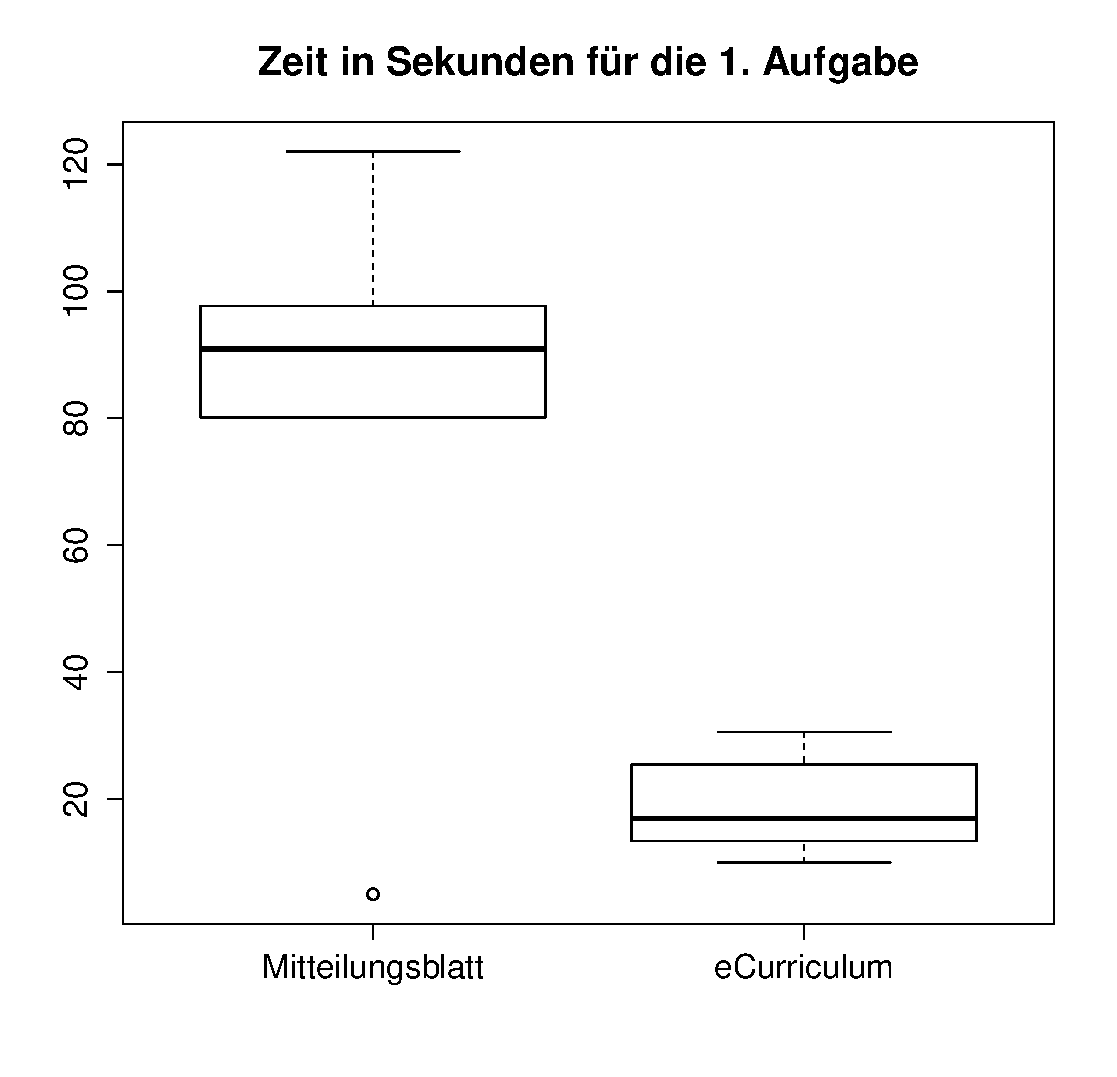
\includegraphics[width=\linewidth]{./Appendix/Plots/Boxplots/a1_boxplot.pdf}
\end{center}

Bei der ersten Aufgabe (Finden der LVs zum Modul VMI) zeigt sich bei Betrachtung des Boxplots über die benötigte Zeit ein deutliches Bild, demzufolge die Bearbeitung der Aufgabe mit dem alten Mitteilungsblatt deutlich mehr Zeit in Anspruch nimmt als mit dem neuen eCurriculum. Ein einziger Ausreißer der Mitteilungsblatt-Zeiten liegt unter allen des eCurriculums, alle anderen Versuchspersonen waren mit dem neuen System schneller.

\begin{center}
 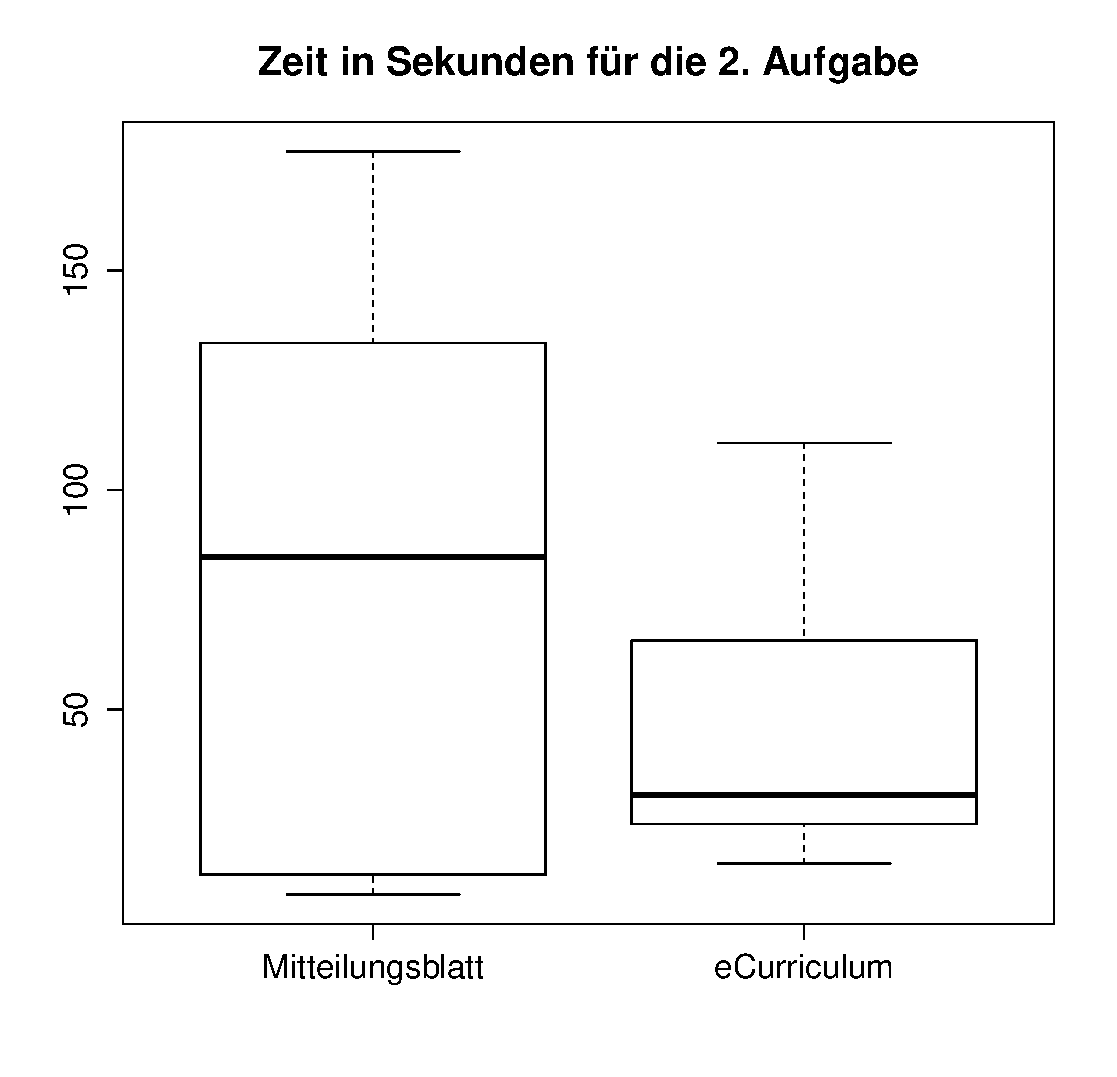
\includegraphics[width=\linewidth]{./Appendix/Plots/Boxplots/a2_boxplot.pdf}
\end{center}

Bei der zweiten Aufgabe (Finden der ECTS-Punkte einer Lehrveranstaltung) zeigt sich bei den Versuchen mit dem Mitteilungsblatt eine deutlich größere Streuung als beim eCurriculum. Zwar liegt der Median beim neuen System deutlich unter dem alten, jedoch gab es auch einige Personen, die mit dem alten System schneller waren.

\begin{center}
 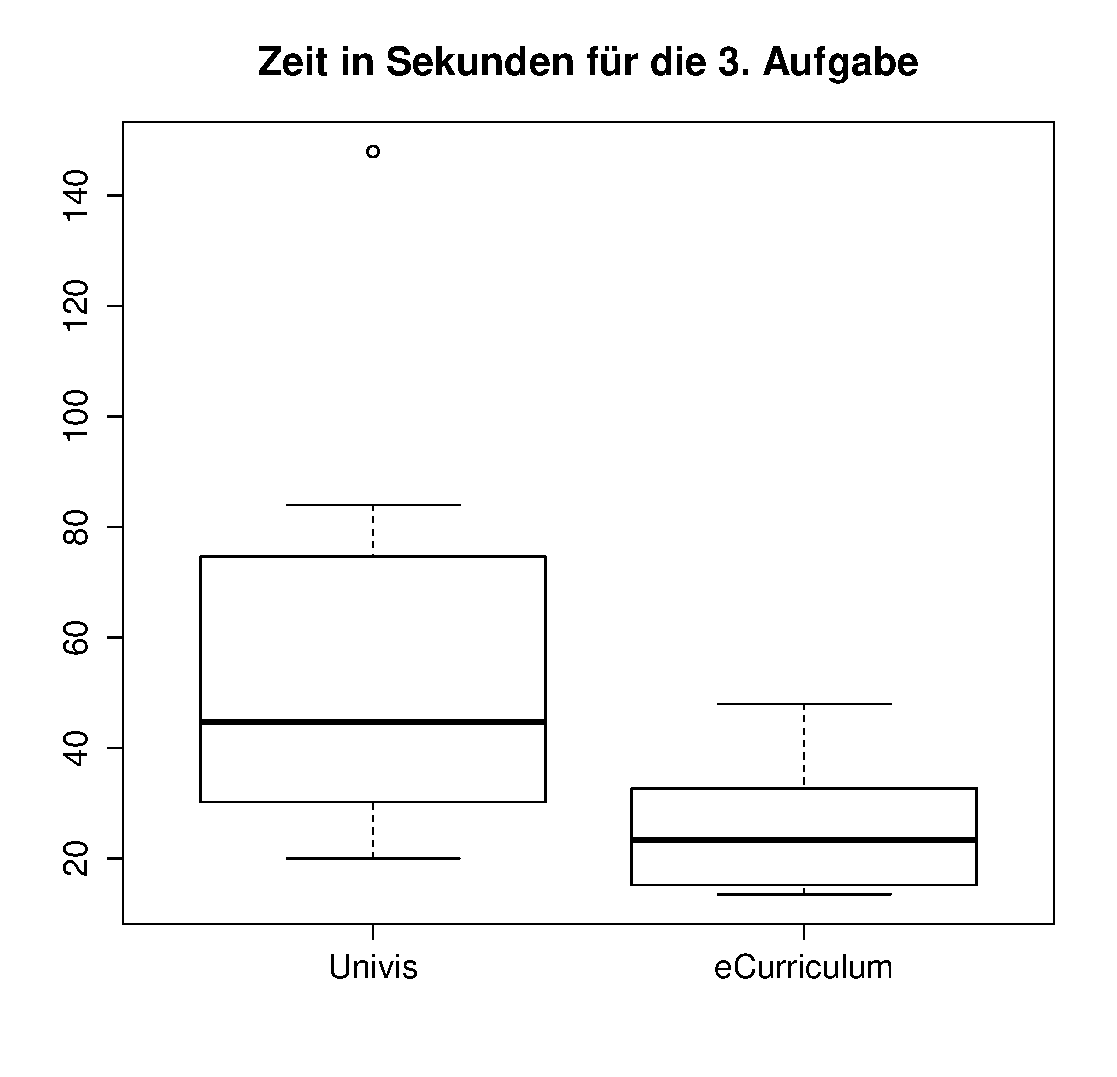
\includegraphics[width=\linewidth]{./Appendix/Plots/Boxplots/a3_boxplot.pdf}
\end{center}

Bei der dritten Aufgabe wurde das Finden einer einzelnen Prüfungsleistung zwischen Univis und eCurriculum verglichen. Hier zeigt sich beim neuen System, dass bei durchschnittlich weniger Bearbeitungszeit auch die Streuung geringer war, viele Versuchspersonen also ähnlich wenig Zeit benötigten.

Beim Univis liegen zwar auch Werte vor, die ähnlich schnell wie im eCurriculum waren, allerdings ist die Streuung bedeutend größer, und es kam auch zu einem sehr auffälligen Ausreißer.

\pagebreak

\subsubsection*{Subjektives Nutzerfeedback} 

\begin{center}
\begin{tabular}{r|r|r|r|r|r|r|r|r}
     & \multicolumn{7}{c}{Mitteilungsblatt} \\ \hline
    Name & einfach & menschlich & verständlich & übersichtlich & innovativ & kreativ & schön & fröhlich \\ \hline
    RL & 2 & 2 & 1 & 7 & 7 & 6 & 7 & 6 \\ \hline
    JM & 5 & 4 & 5 & 6 & 4 & 5 & 6 & 6 \\ \hline
    MS & 5 & 4 & 3 & 6 & 6 & 7 & 5 & 4 \\ \hline
    JF & 3 & 6 & 3 & 4 & 5 & 5 & 4 & 6 \\ \hline
    NM & 5 & 4 & 3 & 6 & 6 & 6 & 6 & 5 \\ \hline
    DK & 2 & 6 & 3 & 6 & 7 & 7 & 5 & 4 \\ \hline
    JB & 4 & 4 & 5 & 3 & 5 & 6 & 7 & 4 \\ \hline
    PH & 2 & 4 & 5 & 1 & 4 & 5 & 7 & 4 \\
\end{tabular}
\end{center}

\begin{center}
\begin{tabular}{r|r|r|r|r|r|r|r|r}
     & \multicolumn{7}{c}{Univis} \\ \hline
    Name & einfach & menschlich & verständlich & übersichtlich & innovativ & kreativ & schön & fröhlich \\ \hline
    RL & 2 & 2 & 1 & 7 & 7 & 6 & 7 & 6 \\ \hline
    JM & 5 & 4 & 5 & 6 & 4 & 5 & 6 & 6 \\ \hline
    MS & 5 & 4 & 3 & 6 & 6 & 7 & 5 & 4 \\ \hline
    JF & 3 & 6 & 3 & 4 & 5 & 5 & 4 & 6 \\ \hline
    NM & 5 & 4 & 3 & 6 & 6 & 6 & 6 & 5 \\ \hline
    DK & 2 & 6 & 3 & 6 & 7 & 7 & 5 & 4 \\ \hline
    JB & 4 & 4 & 5 & 3 & 5 & 6 & 7 & 4 \\ \hline
    PH & 2 & 4 & 5 & 1 & 4 & 5 & 7 & 4 \\
\end{tabular}
\end{center}

\begin{center}
\begin{tabular}{r|r|r|r|r|r|r|r|r}
     & \multicolumn{7}{c}{eCurriculum} \\ \hline
    Name & einfach & menschlich & verständlich & übersichtlich & innovativ & kreativ & schön & fröhlich \\ \hline
    RL & 1 & 2 & 1 & 2 & 3 & 4 & 3 & 3 \\ \hline
    JM & 3 & 4 & 3 & 3 & 4 & 4 & 4 & 4 \\ \hline
    MS & 3 & 3 & 2 & 1 & 2 & 2 & 2 & 2 \\ \hline
    JF & 1 & 2 & 2 & 1 & 1 & 2 & 2 & 2 \\ \hline
    NM & 3 & 3 & 2 & 3 & 4 & 4 & 2 & 4 \\ \hline
    DK & 2 & 3 & 2 & 2 & 3 & 2 & 3 & 3 \\ \hline
    JB & 1 & 3 & 2 & 2 & 5 & 3 & 3 & 4 \\ \hline
    PH & 3 & 3 & 1 & 2 & 5 & 2 & 4 & 1 \\
\end{tabular}
\end{center}

\begin{center}
 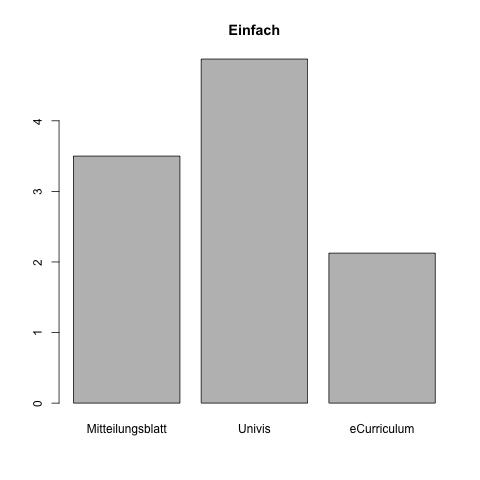
\includegraphics[width=\linewidth]{./Appendix/Plots/Barplots/barplot1.png}
\end{center}
\begin{center}
 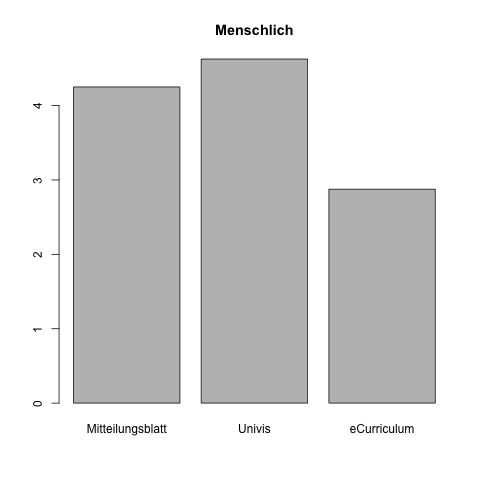
\includegraphics[width=\linewidth]{./Appendix/Plots/Barplots/barplot2.png}
\end{center}
\begin{center}
 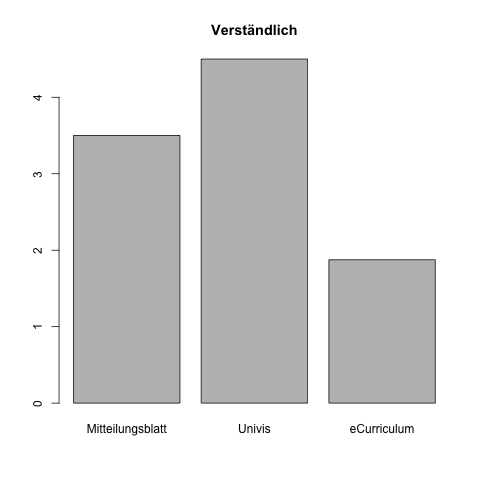
\includegraphics[width=\linewidth]{./Appendix/Plots/Barplots/barplot3.png}
\end{center}
\begin{center}
 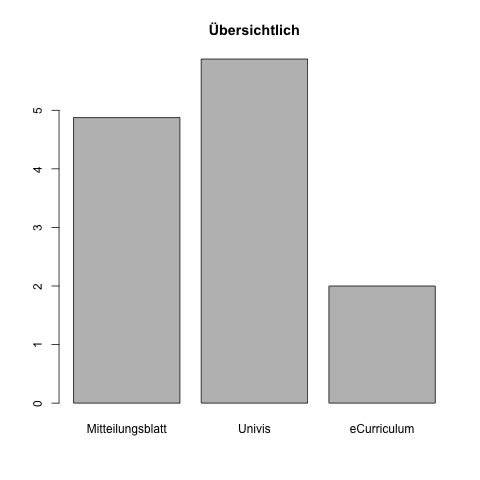
\includegraphics[width=\linewidth]{./Appendix/Plots/Barplots/barplot4.png}
\end{center}
\begin{center}
 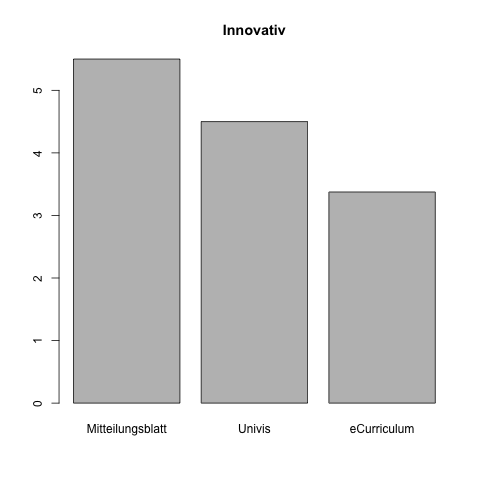
\includegraphics[width=\linewidth]{./Appendix/Plots/Barplots/barplot5.png}
\end{center}
\begin{center}
 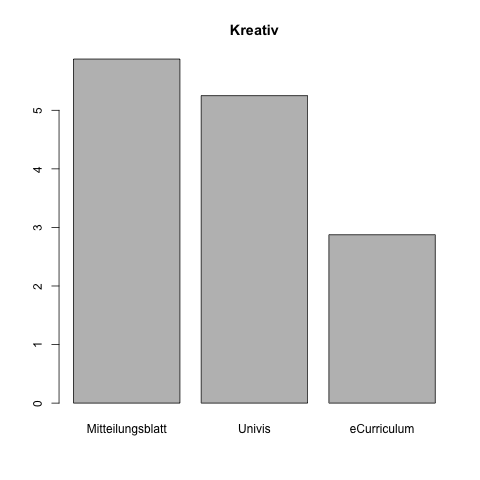
\includegraphics[width=\linewidth]{./Appendix/Plots/Barplots/barplot6.png}
\end{center}
\begin{center}
 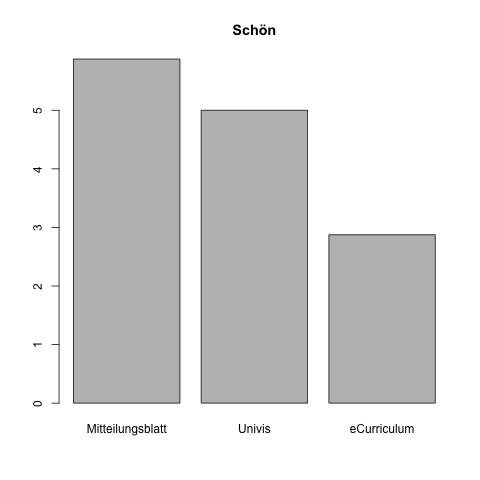
\includegraphics[width=\linewidth]{./Appendix/Plots/Barplots/barplot7.png}
\end{center}
\begin{center}
 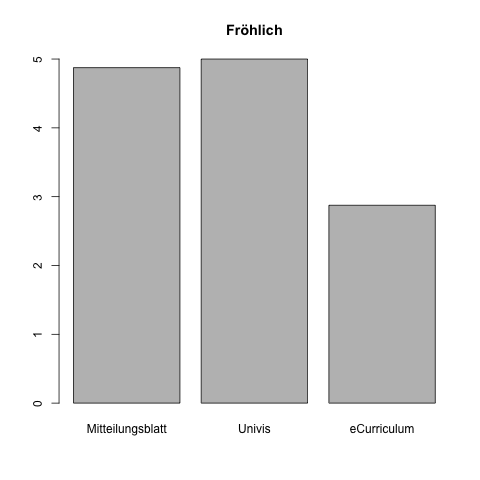
\includegraphics[width=\linewidth]{./Appendix/Plots/Barplots/barplot8.png}
\end{center}

\subsection{Inferenzstatistik}

\subsubsection*{Zeit in Sekunden} 

\subsubsection*{Aufgabe 1:}

\begin{alltt}
Welch Two Sample t-test

data:  a1_mb and a1_ec 
t = 5.1747, df = 7.672, \textbf{p-value = 0.0004839}
alternative hypothesis: true difference in means is greater than 0 
95 percent confidence interval:
 40.88108      Inf 
sample estimates:
mean of x mean of y 
  83.0375   19.0250 
\end{alltt} 

\subsubsection*{Aufgabe 2:}

\begin{alltt}
Welch Two Sample t-test

data:  a2_mb and a2_ec 
t = 1.3532, df = 10.48, \textbf{p-value = 0.1022}
alternative hypothesis: true difference in means is greater than 0 
95 percent confidence interval:
 -11.64372       Inf 
sample estimates:
mean of x mean of y 
  80.7625   45.8125 
\end{alltt} 

\subsubsection*{Aufgabe 3:}

\begin{alltt}
Welch Two Sample t-test

data:  a3_uv and a3_ec 
t = 2.1438, df = 8.156, \textbf{p-value = 0.03187}
alternative hypothesis: true difference in means is greater than 0 
95 percent confidence interval:
 4.434431      Inf 
sample estimates:
mean of x mean of y 
  58.3875   25.4750 
\end{alltt} 

\subsubsection*{Zufriedenheit} 

\begin{alltt}
Welch Two Sample t-test

data:  meansAlt and meansNeu 
t = 6.1818, df = 12.889, \textbf{p-value = 1.721e-05}
alternative hypothesis: true difference in means is greater than 0 
95 percent confidence interval:
 1.61058     Inf 
sample estimates:
mean of x mean of y 
 4.867188  2.609375 
\end{alltt} 

\section{Diskussion}

\subsection{Alternativhypothese 1:  User können mit unserem neu erstellten Interface Aufgaben besser lösen als mit dem alten Interface.} 

Nachdem wir einen Two-Sampled-T-Test durchgeführt haben und uns die p-Value angesehen haben, können wir bei
der 1. Aufgabe sagen, dass bei einem Signfikantsniveau von 95\% die 1. Aufgabe mit dem neuem Interface besser bzw. schneller gelöst werden
kann als mit dem altem Interface, da die Nullhypothese mit einer Fehlerwahrscheinlichkeit von 0,0004839 verworfen werden kann.
\\ \\
Bei der 2. Aufgabe gibt es mit einer p-Value von 0,1022 keinen signifikanten Unterschied. Daher wird die Nullhypothese beibehalten und
mit dem neuem Interface können die Aufgaben nicht signifikant besser gelöst werden.
\\ \\
Bei der 3. Aufgabe kann die Nullhypothese mit einer p-Value von 0,03187 und bei einem Signifikantsniveau von 95\% ebenfalls verworfen werden,
weshalb die Alternativhypothese bewiesen ist und somit die User mit unserem neu erstellten Interface Aufgaben signifikant besser lösen können
als mit dem alten Interface.

\subsection{Alternativhypothese 2: User sind mit unserem neu erstellten Interface zufriedener als mit dem alten Interface. }

Auch hier haben wir wieder einen Two-Sampled-T-Test durchgeführt. Dabei haben wir uns zuerst den Mittelwert je Eigenschaft
berechnet (von ``einfach'' bis ``fröhlich'') und mit diesen Werten dann den T-Test durchgeführt.
\\ \\
Das Ergebnis erhielten wir eine p-Value von 1,721e-05 weshalb man hier auch wieder sagen kann, dass die Nullhypothese bei
einem Signifikantsniveau von 95\% mit einer Fehlerwahrscheinlichkeit von 1,721e-05 verworfen werden kann. Somit ist hier auch wieder unsere
Alternativhypothese bewiesen, welche besagt, dass User mit dem neu erstellten Interface zufriedener sind als mit dem alten Interface.


\section{Appendix}

Enthält:

\begin{itemize}
 \item Beantwortete Fragebögen als .pdf oder .jpg
 \item Daten als .csv-Datei
 \item Plots als .pdf oder .png
 \item R-Skripte für die Plots und die T-Tests
\end{itemize}


\begin{description}
 \item[Datei auf cewebs:] Meilenstein 4 -- Team 1 -- Appendix
\end{description}

\section{Reflexion über das Gesamtprojekt}

\subsection{Kernerkenntnisse und Designempfehlungen aus dem Projekt}

% 
%     Fassen Sie die Kern-Erkenntnisse ihres Projektes zusammen. Beschreiben sie insb. 3-5 konkrete Empfehlungen zu Designverbesserungen, 
%     die sie aus ihrem Gesamtprojekt abgeleitet haben. Diese Zusammenfassung ist als "executive summary" für das UniVis- bzw. das Literacy-team gedacht, 
%     bzw. fuer einen imaginären Kunden, falls sie ein eigenes Thema gewählt haben (max. 1 Seite Text + evtl. Screenshots).

tabellarische Form des Studienplans ist gut angekommen, Mitteilungsblatt in elektronischer Form, Gliederung des Curriculums nach Semester anstatt der eigenartigen
Modulgruppen, direkte Anmeldung zu den Lehrveranstaltungen wenn diese noch nicht absolviert wurden, Studienfortschritt als Anzeige, we are motherfucking awesome

\subsection{Arbeitsverteilung, Kommunikation, Lernprozess und Zufriedenheit}


%     Kurze Beschreibung zu Arbeitsverteilung, Kommunikation, Lernprozess und Zufriedenheit (max 1 Seite). 

Meistens trafen wir uns alle 2 Wochen bzw. dann wenn ein neuer Meilenstein anstand für etwa 3,5 Stunden um den Meilenstein zu besprechen und zu bearbeiten. Die Treffen haben wir uns
dabei entweder direkt in der Einheit oder per Email ausgemacht. Den 1. Meilenstein haben wir dabei bis auf die Erwartungen jedes einzelnen Teammitglieds zusammen gelöst.
Für den 2. Meilenstein trafen wir uns nur für die Erstellung des Low-Fidelity-Prototypen. Der restliche Meilenstein 2 wurde dann in Einzelarbeit, mit Absprache per Mail
gelöst. Bei Meilenstein 3 und 4 haben wir die Fragebögen und die Vorgehensweise für die Interviews
jeweils in unseren Treffen festgelegt. Die Befragung hat dann jeder für sich geführt. Die Auswertung der Interview bzw. des Experiments wurde dann wieder in einem Treffen
durchgeführt.
\\ \\
Zur Arbeitsverteilung ist dabei insgesamt zu sagen, dass viele Aufgaben zusammen gelöst wurden. Der High-Fidelity-Prototyp wurde, bis auf ein paar visuelle Änderungen
und Verbesserungsvorschläge von mir erstellt.
Bei der Durchführung der Interviews und des Experiments haben zwar alle Teammitglieder beigetragen, jedoch wurden die meisten Befragungen von Pascal durchgeführt. Beschreibung
der Prototypen und die Beschreibung und Diskussion der Auswertungen wurde dann wieder von allen Teammitgliedern durchgeführt.
\\ \\
Mitnehmen kann ich aus Human-Computer-Interaction und dem damit verbundenem Projekt, dass die Einbeziehung der späteren Enduser viel zur Usability beiträgt. Durch die Erstellung von Prototypen und anschließende Usability-Interviews wurde man auf viele Usability-Probleme aufmerksam und
konnte diese dann auch verbessern. Auch hat man durch die Durchführung Aspekte die die Usability verbessern und Methoden mit denen die Usability mit Endusern oder auch ohne
getestet werden kann, kennen gelernt.
\\ \\
Insgesamt bin ich mit dem Endprodukt unseres Projektes sehr zufrieden. Was mir jedoch weniger gefallen hat, ist die Dokumentation der Ergebnisse und der Prototypen, da
die Ausformulierungen oft viel Zeit in Anspruch genommen haben. Auch ist es für mich schwierig genug Personen für die Interviews bzw. für das Experiment zu finden, wobei
ich froh war, dass dies dann unser sozialerer Kollege großteils übernommen hat. Interessant fand ich jedoch wiederum die Ergebnisse aus dem Usability-Feedback und aus den Experimenten,
da man hierdurch sieht, wie der High-Fidelity-Prototyp von den Usern gesehen wird.

\end{document}
